\documentclass[11pt]{article}
% Shared preamble for the NSE working-paper series (Mrigank Sahi).
% Usage in each paper: % Shared preamble for the NSE working-paper series (Mrigank Sahi).
% Usage in each paper: % Shared preamble for the NSE working-paper series (Mrigank Sahi).
% Usage in each paper: \input{../common/preamble.tex}
\usepackage[T1]{fontenc}
\usepackage[utf8]{inputenc}
\usepackage{lmodern}
\usepackage{microtype}
\usepackage[a4paper,margin=1in]{geometry}
\usepackage{amsmath,amssymb}
\usepackage{booktabs}
\usepackage{tabularx}
\usepackage{siunitx}
\sisetup{group-separator={,},round-mode=places,round-precision=3}
\usepackage{graphicx}
\usepackage{xcolor}
\usepackage{caption}
\captionsetup{font=small,labelfont=bf}
\usepackage{enumitem}
\setlist{nosep,leftmargin=*}
\usepackage[framemethod=TikZ]{mdframed}
\usepackage[numbers,sort&compress]{natbib}
\usepackage[colorlinks=true,linkcolor=black,citecolor=blue!50!black,urlcolor=blue!50!black]{hyperref}

\newcommand{\ghbase}{https://github.com/mriganksahi-beep}
\newcommand{\authorline}{Mrigank Sahi\\\small Independent Researcher, New Delhi\\\small\texttt{mriganksahi@gmail.com}}

% Standard disclosure box. Every paper fills all five fields.
% #1 sample/period status, #2 position in test tally, #3 costs,
% #4 point-in-time limits, #5 anything else the reader must know
\newcommand{\caveatsbox}[5]{%
\begin{mdframed}[backgroundcolor=gray!8,linecolor=gray!50,innertopmargin=6pt,innerbottommargin=6pt]
\small\textbf{Read before interpreting results.}
\begin{itemize}
\item \textbf{Sample.} #1
\item \textbf{Multiple testing.} #2
\item \textbf{Costs.} #3
\item \textbf{Point-in-time universe.} #4
\item \textbf{Other.} #5
\end{itemize}
\end{mdframed}}

% Standard AI-assistance statement (identical across the series).
\newcommand{\aistatement}{%
\paragraph{Use of AI tools.} Code for this project was written with the assistance of
an AI coding assistant (Anthropic's Claude), working to specifications set by the
author, and the manuscript was drafted with the same assistance. The author designed
the research questions and decision rules and ran the main analyses. Some diagnostics
added during revision were computed by the assistant from archived run outputs; these
are labelled as revision diagnostics in the text. The author reviewed all code and
text and takes full responsibility for the content.}

% Standard data/code availability statement.
\newcommand{\availability}[1]{%
\paragraph{Data and code availability.} Code: \url{#1}. The point-in-time panel
construction is documented in \url{\ghbase/indian-equity-research/tree/main/data_pipeline}.
Price data from Yahoo Finance and index-membership snapshots from a licensed vendor
are not redistributed; the repository contains the scripts to rebuild the panel.}

% Placeholder for anything awaiting the author's confirmation. Renders red so it
% cannot survive into a posted PDF unnoticed.
\newcommand{\verify}[1]{\textcolor{red}{\textbf{[VERIFY: #1]}}}

\usepackage[T1]{fontenc}
\usepackage[utf8]{inputenc}
\usepackage{lmodern}
\usepackage{microtype}
\usepackage[a4paper,margin=1in]{geometry}
\usepackage{amsmath,amssymb}
\usepackage{booktabs}
\usepackage{tabularx}
\usepackage{siunitx}
\sisetup{group-separator={,},round-mode=places,round-precision=3}
\usepackage{graphicx}
\usepackage{xcolor}
\usepackage{caption}
\captionsetup{font=small,labelfont=bf}
\usepackage{enumitem}
\setlist{nosep,leftmargin=*}
\usepackage[framemethod=TikZ]{mdframed}
\usepackage[numbers,sort&compress]{natbib}
\usepackage[colorlinks=true,linkcolor=black,citecolor=blue!50!black,urlcolor=blue!50!black]{hyperref}

\newcommand{\ghbase}{https://github.com/mriganksahi-beep}
\newcommand{\authorline}{Mrigank Sahi\\\small Independent Researcher, New Delhi\\\small\texttt{mriganksahi@gmail.com}}

% Standard disclosure box. Every paper fills all five fields.
% #1 sample/period status, #2 position in test tally, #3 costs,
% #4 point-in-time limits, #5 anything else the reader must know
\newcommand{\caveatsbox}[5]{%
\begin{mdframed}[backgroundcolor=gray!8,linecolor=gray!50,innertopmargin=6pt,innerbottommargin=6pt]
\small\textbf{Read before interpreting results.}
\begin{itemize}
\item \textbf{Sample.} #1
\item \textbf{Multiple testing.} #2
\item \textbf{Costs.} #3
\item \textbf{Point-in-time universe.} #4
\item \textbf{Other.} #5
\end{itemize}
\end{mdframed}}

% Standard AI-assistance statement (identical across the series).
\newcommand{\aistatement}{%
\paragraph{Use of AI tools.} Code for this project was written with the assistance of
an AI coding assistant (Anthropic's Claude), working to specifications set by the
author, and the manuscript was drafted with the same assistance. The author designed
the research questions and decision rules and ran the main analyses. Some diagnostics
added during revision were computed by the assistant from archived run outputs; these
are labelled as revision diagnostics in the text. The author reviewed all code and
text and takes full responsibility for the content.}

% Standard data/code availability statement.
\newcommand{\availability}[1]{%
\paragraph{Data and code availability.} Code: \url{#1}. The point-in-time panel
construction is documented in \url{\ghbase/indian-equity-research/tree/main/data_pipeline}.
Price data from Yahoo Finance and index-membership snapshots from a licensed vendor
are not redistributed; the repository contains the scripts to rebuild the panel.}

% Placeholder for anything awaiting the author's confirmation. Renders red so it
% cannot survive into a posted PDF unnoticed.
\newcommand{\verify}[1]{\textcolor{red}{\textbf{[VERIFY: #1]}}}

\usepackage[T1]{fontenc}
\usepackage[utf8]{inputenc}
\usepackage{lmodern}
\usepackage{microtype}
\usepackage[a4paper,margin=1in]{geometry}
\usepackage{amsmath,amssymb}
\usepackage{booktabs}
\usepackage{tabularx}
\usepackage{siunitx}
\sisetup{group-separator={,},round-mode=places,round-precision=3}
\usepackage{graphicx}
\usepackage{xcolor}
\usepackage{caption}
\captionsetup{font=small,labelfont=bf}
\usepackage{enumitem}
\setlist{nosep,leftmargin=*}
\usepackage[framemethod=TikZ]{mdframed}
\usepackage[numbers,sort&compress]{natbib}
\usepackage[colorlinks=true,linkcolor=black,citecolor=blue!50!black,urlcolor=blue!50!black]{hyperref}

\newcommand{\ghbase}{https://github.com/mriganksahi-beep}
\newcommand{\authorline}{Mrigank Sahi\\\small Independent Researcher, New Delhi\\\small\texttt{mriganksahi@gmail.com}}

% Standard disclosure box. Every paper fills all five fields.
% #1 sample/period status, #2 position in test tally, #3 costs,
% #4 point-in-time limits, #5 anything else the reader must know
\newcommand{\caveatsbox}[5]{%
\begin{mdframed}[backgroundcolor=gray!8,linecolor=gray!50,innertopmargin=6pt,innerbottommargin=6pt]
\small\textbf{Read before interpreting results.}
\begin{itemize}
\item \textbf{Sample.} #1
\item \textbf{Multiple testing.} #2
\item \textbf{Costs.} #3
\item \textbf{Point-in-time universe.} #4
\item \textbf{Other.} #5
\end{itemize}
\end{mdframed}}

% Standard AI-assistance statement (identical across the series).
\newcommand{\aistatement}{%
\paragraph{Use of AI tools.} Code for this project was written with the assistance of
an AI coding assistant (Anthropic's Claude), working to specifications set by the
author, and the manuscript was drafted with the same assistance. The author designed
the research questions and decision rules and ran the main analyses. Some diagnostics
added during revision were computed by the assistant from archived run outputs; these
are labelled as revision diagnostics in the text. The author reviewed all code and
text and takes full responsibility for the content.}

% Standard data/code availability statement.
\newcommand{\availability}[1]{%
\paragraph{Data and code availability.} Code: \url{#1}. The point-in-time panel
construction is documented in \url{\ghbase/indian-equity-research/tree/main/data_pipeline}.
Price data from Yahoo Finance and index-membership snapshots from a licensed vendor
are not redistributed; the repository contains the scripts to rebuild the panel.}

% Placeholder for anything awaiting the author's confirmation. Renders red so it
% cannot survive into a posted PDF unnoticed.
\newcommand{\verify}[1]{\textcolor{red}{\textbf{[VERIFY: #1]}}}

\usepackage{xurl}

\title{Path Texture and the Cross-Section of Indian Equity Returns:\\
Permutation Entropy and the Variance Ratio}
\author{\authorline}
\date{October 2026}

\begin{document}
\maketitle

\begin{abstract}
\noindent Two measures of the \emph{shape} of a stock's recent daily return path were
tested as cross-sectional return predictors on a snapshot-based approximation to the
Nifty~500: normalized permutation entropy (order 4) and the 21-day Lo--MacKinlay
variance ratio, both over a 232-row window. The variance ratio stood in for a planned
wavelet measure that was never built. Each test had a registered first gate. Neither
measure passed it: Fama--MacBeth Newey--West $t$-statistics were $-0.29$ (entropy) and
$-0.41$ (variance ratio) even before controls, and all 95\% intervals include zero. A
revision diagnostic finds that most stock-months have entropy close to the finite-sample
i.i.d.\ benchmark. Simulated noise of the same length reproduces about two-thirds of the
cross-sectional entropy variance. The entropy test used 2011--2026 data including 2022
onward; a post hoc 2011--2021 re-estimate also fails the gate.
\end{abstract}

\caveatsbox
{Test M7 (entropy) used monthly rebalances 2011-01 to 2026-06, including 2022 onward.
Tests D (variance ratio) and C (appendix) used 2010--2021 only; Test~D's last forward
window reads 21 trading days of January 2022, and a strict re-estimate that drops it is
reported. No result here is validated on untouched data.}
{Legacy ledger: M7 is item 29 (the momentum-enhancement batch's internal count,
\citet{sahi_momentum}); the Test~C gate and its diagnostics are 30 and 31; the Test~D gate
is 32. The revision diagnostics in Sections~\ref{sec:diag}--\ref{sec:repro} are post hoc,
are not registered tests and are not in that count. No multiplicity adjustment was
applied because no test passed.}
{No portfolio was formed. All statistics are gross cross-sectional coefficients or
correlations.}
{Membership is a snapshot-based point-in-time approximation built from semi-annual
Nifty~500 lists; the 2018-06-30 snapshot is truncated (about 353 instead of about 500
names, carried forward from 2017-12-31), so up to about 22\% of names may be
misclassified in July--December 2018.}
{No wavelet transform was computed. Seven development-period month-ends are absent or
dropped (Section~\ref{sec:data}); a calendar-corrected rerun is pending and could change
sample counts and estimates slightly. All 95\% intervals were added during drafting or
revision.}

\section{Introduction}

Momentum ranks stocks by the \emph{magnitude} of their past return. A natural follow-up
question is whether the \emph{texture} of the path also matters: whether stocks reached
the same 12-month return smoothly or in jumps, and whether their movement was concentrated
at slow or fast horizons. The ``frog-in-the-pan'' result of \citet{da2014} is the
best-known version of this idea. Permutation entropy \citep{bandt2002} and multiscale
variance measures are model-free ways to describe path shape.

This paper reports two gated tests of the idea on Indian equities. Test~M7, run inside a
momentum-enhancement batch \citep{sahi_momentum}, asked whether, at equal 12--1 momentum,
stocks with low permutation entropy (smooth paths) later outperformed stocks with high
entropy (jumpy paths). Test~D asked whether the balance between slow-scale and fast-scale
movement, measured by the variance ratio, predicted forward returns independently of
volatility. In both tests, cheap checks had to pass before any portfolio sort was allowed.

\paragraph{Contribution.} For the two specified measures, on daily returns over a 232-row
window, neither passed its registered first forward-return gate. The 95\% intervals rule
out large effects more clearly than small ones. The diagnostics show that the entropy
measure is close to its finite-sample i.i.d.\ reference for most stock-months, and that
much of the cross-sectional variation in either measure is of the size that sampling noise
alone produces. This is consistent with measurement noise being a substantial part of
the story, but it does not prove that noise is the only reason for the null. The paper is
complementary to \citet{sahi_irfa}, which studies regime-dependent momentum and reversal
ICs and does not use path-shape measures.

\section{Data and universe}
\label{sec:data}

All tests used one daily panel (1,069 tickers, 2010-01-04 to 2026-07-10; file
\nolinkurl{feature_panel_with_pit_v2_2026-07-24}), documented in
\url{\ghbase/India-Equity-Research/tree/main/data_pipeline}. Daily returns are close-to-close on the ticker's prior
trading row. Placeholder rows that the data vendor creates on non-trading days were
masked first. \texttt{realized\_vol\_60} is the annualized 60-row standard deviation of
daily returns, turnover is volume $\times$ close, and Amihud illiquidity is a monthly mean
of $|r|/\text{turnover}$.

A rebalance date $t$ is the last row of each calendar month in the panel's date index.
A stock is eligible if its membership flag equals 1 on $t$, it is not one of eight tickers
with known corporate-action splices, it has a complete 12--1 momentum window, and at least
200 of the 232 rows from $t-252$ to $t-21$ (inclusive) have a return. The 252-row lookback
with a 21-row skip leaves this 232-row window, and both path measures use only it. The
forward return compounds rows $t+1$ to $t+21$. Months with fewer than 100 eligible names
are dropped.

\paragraph{Skipped months.} Across 2011--2021, seven month-ends are absent or dropped in
both the entropy and the variance-ratio panels. Five months have no rebalance row at all:
2011-08, 2014-08, 2016-10, 2018-03 and 2020-11. Their month-ends coincide with exchange
holidays on which the panel's date index carried rows that most tickers left blank. Two
further months are below the 100-name floor. 2015-02-28 (56 names) was a genuine Saturday
session held for the Union Budget, and its cross-section is thin. 2019-03-29 (30 names) is
unexplained. In the full M7 sample, 2025-03, 2025-04 and 2025-05 are also dropped because
\texttt{realized\_vol\_60} is missing for nearly all names after a vendor-failure day on
2025-03-18. A calendar-corrected rerun of the panel is pending. All sample counts and
estimates that it could change are listed in \texttt{RERUN\_DEPENDENT.md}. The development
slice used for M7 diagnostics, which equals the Test~D panel, has 59,184 stock-months on
865 tickers.

\section{Method}
\label{sec:method}

\subsection{Permutation entropy}

Each run of $m$ consecutive returns is mapped to its ordinal pattern, the order that sorts
it.\footnote{For $m=4$, the returns $(0.2\%, -1.0\%, 0.5\%, 0.1\%)$ sort as positions
$(2,4,1,3)$. That pattern is one of $4!=24$ possible patterns.} With $p_\pi$ the share
of pattern $\pi$ among the $n-m+1$ windows \citep{bandt2002},
\begin{equation}
  \mathrm{PE}_m=-\frac{1}{\ln m!}\sum_\pi p_\pi\ln p_\pi\in[0,1].
\end{equation}
M7 used $m=4$, $\tau=1$ (primary) and $m=3$ as a robustness variant. A monotone path uses
one pattern ($\mathrm{PE}=0$). For an i.i.d.\ continuous series, every pattern is equally
likely whatever the marginal distribution. Even so, a finite series of about 229 windows
has PE strictly below 1, because the 24 empirical frequencies fluctuate around $1/24$. The
relevant benchmark is therefore the finite-sample i.i.d.\ distribution, not 1.
Ties (repeated values, such as zero-return days) are ordered by \texttt{numpy.argsort}'s
default sort, which is deterministic but not stable, so tied values are not guaranteed to
keep their time order. Section~\ref{sec:ties} tests sensitivity to this rule. Sample entropy \citep{richman2000} with $m=2$ and
$r=0.2\hat\sigma$, and the DGW control (the share of positive days), use the same window.

\subsection{Variance ratio as a stand-in for wavelet scale energy}

Test~D was motivated by a wavelet idea: the share of path energy at coarse scales. Total
wavelet energy equals the sample variance, so raw band energies are volatility in disguise.
The design therefore gated on a scale-free quantity that addresses a related question,
the overlapping variance ratio \citep{lo1988}:
\begin{equation}
  \widehat{\mathrm{VR}}(q)=\frac{\sum_{j=q}^{n}\big(X_j-X_{j-q}-q\hat\mu\big)^2\big/\big[q(n-q+1)(1-q/n)\big]}
  {\sum_{t=1}^{n}(r_t-\hat\mu)^2/(n-1)},\qquad X_j=\sum_{t\le j}r_t,
\end{equation}
with $q=21$ and no further finite-sample correction. $\mathrm{VR}(q)>1$ indicates positive
serial dependence at the 21-day aggregation, and $\mathrm{VR}(q)<1$ indicates negative
dependence. The variance ratio is not a wavelet energy share. Its pre-build checks on
simulated series of length 1,000 returned 1.87 for a trending process, 0.40 for a
mean-reverting one and 1.03 for a random walk. A wavelet build (maximal-overlap transform,
Daubechies least-asymmetric filter of length 8) was planned only if all three gates passed.
It never ran, and no conclusion about wavelets follows from this paper.

\subsection{Gate design and inference}

Table~\ref{tab:gates} lists the gates. A gate that ran and missed its threshold
\emph{failed}. A gate that never ran because an earlier one failed is \emph{not
reached}. Gate-1 statistics are monthly Fama--MacBeth regressions of the 21-day forward
return on cross-sectionally $z$-scored regressors. Inference uses the time series of
monthly coefficients, with a Newey--West (Bartlett, lag~6) standard error. The decision
used the \emph{controlled} coefficient. The \emph{uncontrolled} coefficient was also
recorded, and its definition differs between tests. In M7 it comes from a regression on
entropy and momentum, because the hypothesis is stated ``at equal 12--1 return''. In D it
comes from a regression on VR alone. The uncontrolled coefficient separates two
situations: a signal that the control explains away, and a signal that was never there.

\begin{table}[t]
\centering\small
\caption{Registered gate chains. FM = monthly Fama--MacBeth; $t$ = Newey--West (lag 6).
Rules are as written in the notebooks before the gate cells ran.}
\label{tab:gates}
\begin{tabularx}{\textwidth}{@{}l l X l@{}}
\toprule
Test & Gate & Pass rule & Outcome \\
\midrule
M7 & 1 Distinctness & FM: $\mathrm{PE}_4$ coefficient with momentum and DGW controls has $|t|>2$ and the same sign as the uncontrolled coefficient & \textbf{failed} ($t=-0.12$) \\
   & 2 Volatility & gate 1 plus $\log$ RV60 & not reached \\
   & 3 Stability & block-bootstrap rank stability $>0.6$ & not reached \\
   & 4 Performance & momentum $\times$ entropy double-sort & not computed \\
\addlinespace
D  & 1 Vol-orthogonalization & FM: VR(21) residual on $\log$ RV60, with $\log$ RV60, momentum and $\log$ Amihud controls, has $|t|>2$ and the same sign & \textbf{failed} ($t=-0.23$) \\
   & 2 Dispersion & mean monthly p10--p90 spread of VR(21) $>0.30$ & not reached \\
   & 3 Stability & block-bootstrap rank stability $>0.6$ & not reached \\
   & -- Wavelet build & MODWT, LA8 & not built \\
\bottomrule
\end{tabularx}
\end{table}

\section{Results}
\label{sec:results}

Table~\ref{tab:fm} reports gate~1. The ``as run'' rows were reproduced exactly from the
cached panels with the notebooks' code. Coefficients are 21-day returns per one
cross-sectional standard deviation of the signal; for example, $-0.00059$ means $-0.059$
percentage points per month.

\begin{table}[t]
\centering\footnotesize\setlength{\tabcolsep}{4pt}
\caption{Gate-1 Fama--MacBeth results. $T$ = months. All intervals are post hoc: 95\%,
coefficient $\pm1.96$ Newey--West standard errors. A circular block bootstrap of the
monthly series (block 6, 10,000 draws) gives endpoints within $\pm0.0002$ of these.
Rows marked $\dagger$ are post hoc sample restrictions added after the as-run result was
seen.}
\label{tab:fm}
\begin{tabular}{@{}l l r r r l@{}}
\toprule
Sample & Regressors & Coef. & NW $t$ & $T$ & 95\% interval \\
\midrule
M7, 2011--2026 (as run) & PE, mom.\ (uncontrolled) & $-0.00012$ & $-0.29$ & 176 & $[-0.00089,\ 0.00066]$ \\
                        & PE, mom., DGW (gate) & $-0.00005$ & $-0.12$ & 176 & $[-0.00083,\ 0.00073]$ \\
M7, 2011--2021$^\dagger$ & PE, mom.\ (uncontrolled) & $+0.00039$ & $+0.88$ & 125 & $[-0.00047,\ 0.00124]$ \\
                        & PE, mom., DGW (gate) & $+0.00048$ & $+1.09$ & 125 & $[-0.00038,\ 0.00134]$ \\
\addlinespace
D, 2011--2021 (as run)  & VR(21) (uncontrolled) & $-0.00059$ & $-0.41$ & 125 & $[-0.0034,\ 0.0022]$ \\
                        & VR resid., RV, mom., Amihud (gate) & $-0.00028$ & $-0.23$ & 125 & $[-0.0027,\ 0.0021]$ \\
D, to 2021-11$^\dagger$  & VR(21) (uncontrolled) & $-0.00066$ & $-0.46$ & 124 & -- \\
                        & VR resid., RV, mom., Amihud (gate) & $-0.00034$ & $-0.28$ & 124 & $[-0.0027,\ 0.0021]$ \\
\bottomrule
\end{tabular}
\end{table}

\paragraph{M7.} As run, the entropy coefficient was $-0.00012$ ($t=-0.29$) with momentum
controlled, and $-0.00005$ ($t=-0.12$) after DGW was added, so gate~1 failed. The
notebook's automatic label (``reinvented frog-in-the-pan'') describes this failure
inaccurately. DGW did not remove a signal, because the uncontrolled coefficient was already
indistinguishable from zero. The sample includes 2022 onward. The 2011--2021 re-estimate
was run after the full-sample result had been seen, so it is a restricted-sample
sensitivity and not a confirmatory test. Its coefficients change sign ($t=0.88$ and $1.09$)
but still fail the gate.

\paragraph{D.} The uncontrolled VR coefficient was $-0.00059$ ($t=-0.41$), and the gate
coefficient was $-0.00028$ ($t=-0.23$). Gate~1 failed, so gates~2 and~3 were not
reached and the wavelet build did not run. Test~D's last rebalance, 2021-12-31, has a
forward window inside January 2022. Dropping it leaves 124 months, with an uncontrolled
$t$ of $-0.46$ and a gate $t$ of $-0.28$, so the conclusion does not change.

\paragraph{Precision.} Every interval in Table~\ref{tab:fm} includes zero. The data rule
out effects larger than about 0.13 percentage points per month per standard deviation for
entropy and about 0.3 for the variance ratio. They do not distinguish a zero effect from
smaller ones. The appropriate reading is ``not detected at the available precision''.

\section{Revision diagnostics}
\label{sec:diag}

None of the analyses in this section was registered. Simulated nulls use fixed seeds
(Table~\ref{tab:repro}).

\subsection{Entropy against its finite-sample i.i.d.\ benchmark}

\begin{figure}[t]
\centering
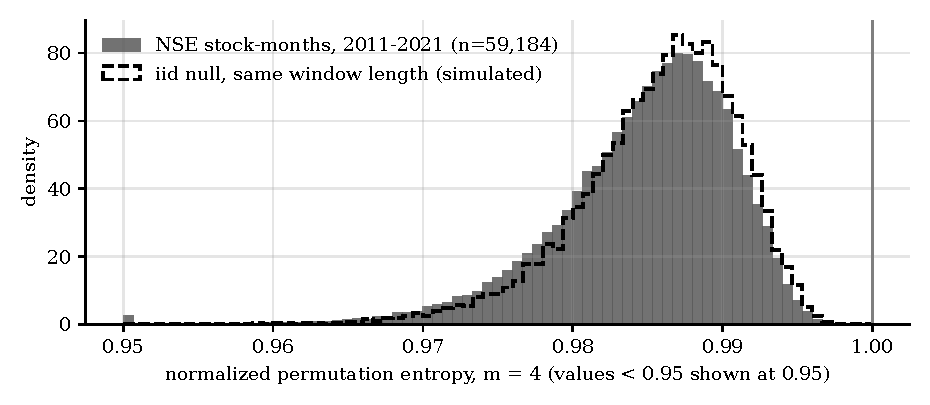
\includegraphics[width=\textwidth]{figures/fig1_pe_distribution.pdf}
\caption{$\mathrm{PE}_4$ for all 59,184 eligible stock-months, 2011--2021 (bars), and
20,000 simulated i.i.d.\ Gaussian series of length 232 (dashed). Because ordinal patterns
of an i.i.d.\ continuous series do not depend on its distribution, the simulated null
depends only on $n$ and $m$. Simulated series contain no ties.}
\label{fig:pe}
\end{figure}

The 1st, 50th and 99th percentiles of $\mathrm{PE}_4$ are 0.966, 0.986 and 0.995.
99.8\% of stock-months are at or above 0.95, and the minimum is 0.805. The simulated
i.i.d.\ benchmark has mean 0.986 and standard deviation 0.0053, and 98.5\% of observed
values lie inside its central 99\% band (Figure~\ref{fig:pe}). The mean within-month
cross-sectional standard deviation of observed PE is 0.0065. The i.i.d.\ sampling
variance is about 65\% of the observed cross-sectional variance. So, for this estimator,
window and sample, most stock-months are close to i.i.d.\ in ordinal terms, and most of the
spread that M7 would have ranked on is of the size produced by sampling noise. This
says nothing about the full return process: amplitude-based sample entropy (median 1.88)
is clearly below its own i.i.d.\ reference (2.20, 500 draws), so the series are not i.i.d.

\subsection{The low tail: ties and price discreteness}
\label{sec:ties}

Only 96 development stock-months on 18 tickers have $\mathrm{PE}_4<0.95$. Within each
month, PE is $z$-scored before the regression, and the lowest value reaches $z=-17.3$, so
these few observations have high leverage. To inspect them, daily returns were rebuilt from
the raw price files for 35 tickers: the 15 with the lowest minimum PE, which cover 97\% of
the sub-0.95 stock-months, and 20 tickers drawn at random. The rebuilt returns reproduce
the cached PE exactly for all 2,189 stock-months. Three tie treatments were then compared:
the original sort order, random tie-breaking (20 jittered draws), and dropping zero-return
days.

The results are as follows (Figure~\ref{fig:ties}). Ties are common in the low tail: 52\% of
its stock-months contain at least one tied four-day window, against 15\% for the random
tickers. Tie-breaking order still barely matters: the median PE change is zero in both
groups. Of the 93 inspected stock-months below 0.95, only 4\% rise above 0.95 under random
tie-breaking, and the minimum moves from 0.805 to 0.817. The extreme case, SHREEASHTA at
2013-07-31, had 19.8\% zero-return days, ties in 26\% of its windows, and a median price of
Rs~2.25 in the window. Dropping its zero days lowers PE further, to 0.681. Price is the
common feature: 73\% of the sub-0.95 stock-months have a window median price below
Rs~10 (median Rs~3.55, against Rs~128 for the random tickers). With a fixed tick
size, returns at such prices take only a few discrete values. The low tail therefore looks
like genuine ordinal structure in very low-priced stocks, consistent with price
discreteness or bid--ask bounce, rather than an artefact of the tie rule. This explanation
was not tested further. One low-tail ticker (GBGLOBAL) shows window prices near
Rs~88,600, which suggests a price-scale error in the raw file; it was not corrected.

\begin{figure}[t]
\centering
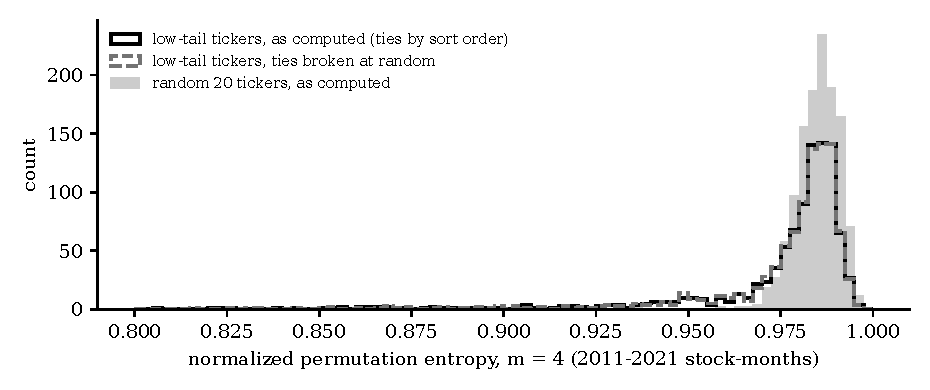
\includegraphics[width=\textwidth]{figures/fig4_ties.pdf}
\caption{Revision diagnostic. $\mathrm{PE}_4$ for 965 stock-months of the 15 low-tail
tickers under the original tie rule (solid) and with ties broken at random (dashed),
against 1,235 stock-months of 20 randomly drawn tickers (shaded), 2011--2021.}
\label{fig:ties}
\end{figure}

\paragraph{Effect on the M7 gate.} Re-estimating the full panel's tie treatment would
need the full return panel, which was not available for this revision. Instead, the gate
was rerun on the cached panel in two ways that remove the tail's leverage. Dropping
stock-months with $\mathrm{PE}_4<0.95$ gives gate $t$-statistics of $-0.83$ (2011--2026)
and $+0.38$ (2011--2021). Replacing $z(\mathrm{PE})$ with $z(\text{rank})$ gives $-1.11$
and $+0.47$. Every variant still fails the $|t|>2$ rule.

\subsection{Variance ratios and the random-walk probe}

\begin{figure}[t]
\centering
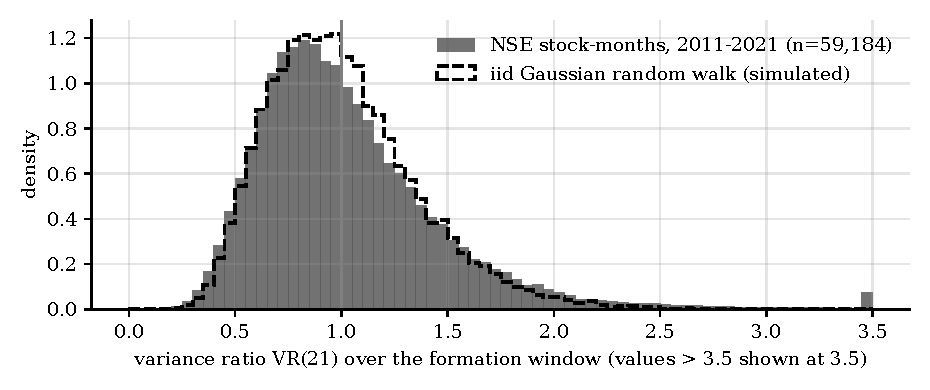
\includegraphics[width=\textwidth]{figures/fig2_vr_distribution.pdf}
\caption{VR(21) for all Test~D stock-months, 2011--2021 (bars), and 20,000 Gaussian random
walks of length 232 passed through the same estimator (dashed).}
\label{fig:vr}
\end{figure}

The observed median VR(21) is 0.950, and the simulated random-walk median is 0.958
(Figure~\ref{fig:vr}). With 20,000 draws, the random-walk mean is 1.00 and the standard
deviation 0.35 at length 232, and 1.00 and 0.34 at length 252. The source notes report a
random-walk mean of 0.95 and standard deviation 0.30 at length 252 over 200 seeds, and
describe the estimator as unbiased. The original simulation code was not found, so that
figure could not be reproduced as the same experiment. A reconstruction with Gaussian
i.i.d.\ returns, length 252 and seeds 0--199 gives 0.949 and 0.297, matching it to two
decimals. With 100 times as many draws, the mean is 1.00. The 0.95 is therefore
consistent with Monte Carlo error over 200 draws (standard error about 0.02). It is not
evidence that the estimator is unbiased, and that claim is withdrawn. Under the Gaussian
random-walk null, sampling noise accounts for about 53\% of the observed cross-sectional
variance of VR (mean within-month standard deviation 0.47). Heavy tails and volatility
clustering would raise that share.

\subsection{Estimator stability and agreement}

M7 measured rank stability as the Spearman correlation between a month's $\mathrm{PE}_4$
ranking and the ranking recomputed on block-bootstrapped paths (20-day blocks, 50
resamples). The value was 0.440 over 12 months (range 0.411--0.477), against a bar of 0.6.
Three of the 12 months fall in 2022 onward, and the nine development months average
0.444. $\mathrm{PE}_3$ and $\mathrm{PE}_4$ correlate at 0.770. In the notebook's check
month, sample entropy correlated with $\mathrm{PE}_4$ at only 0.06--0.11 across its
$(m,r)$ grid, so the two disorder measures rank stocks almost independently. The source
note's statement that they ``agree'' is not supported. Volatility clustering is one
possible reason why sample entropy departs from i.i.d.\ while PE does not; this is a
hypothesis for future work.

\section{What this paper does not establish}

The paper does not show that path shape is uninformative in general. Only two estimators
were tested, at one frequency (daily), over one window (232 rows), on one approximate
universe. It does not test wavelet scale energy. It does not show that NSE returns are
i.i.d.: the entropy diagnostic concerns ordinal patterns only, and sample entropy points
the other way. It does not establish a zero effect, because effects smaller than the
interval half-widths are not excluded. Nothing here validates out of sample: the entropy
test used 2022 onward, and the restricted re-estimates were chosen after the full-sample
result was known.

\section{Limitations}
\label{sec:limits}

\begin{itemize}
\item \textbf{Use of 2022 onward.} M7 read 2022--2026. A 2010--2021/2022--2026 split was
already defined in earlier batch notebooks \citep{sahi_momentum}, but a code-level wall
first appears in the Test~C notebook (2026-08-08), after M7 (2026-08-04).
\item \textbf{Gate~2 calibration (Test~D).} The rule compared a p10--p90 range with a noise
standard deviation of 0.30. A normal variable with that standard deviation already has a
p10--p90 range of about 0.77, so the gate was not a like-for-like comparison. Future gates
should use simulated null quantiles of the same statistic. Gate~2 never ran, so this flaw
weakens the planned chain but does not change the gate-1 result.
\item \textbf{Tie sensitivity of the full gate} was examined on a 35-ticker subset and
through tail-robust re-estimates, not by rebuilding the full panel with an alternative tie
rule.
\item \textbf{Calendar defect and data quality.} The months listed in Section~\ref{sec:data}
await a calendar-corrected rerun. The 2025 volatility gap affects only the M7 full sample.
The stale-price family of tickers has no filter yet.
\item \textbf{Universe.} Membership comes from semi-annual snapshots, and the 2018H2
snapshot is truncated.
\end{itemize}

\section{Conclusion}

For the specified daily-return window and the two registered measures, neither
permutation entropy nor the 21-day variance ratio passed its first forward-return gate.
Most observed entropy values lie near the finite-sample i.i.d.\ ordinal-pattern benchmark.
The few that do not are concentrated in very low-priced stocks and are not an artefact of
tie ordering. Simulated nulls suggest that sampling variation accounts for a substantial
share of the cross-sectional dispersion in both measures. These diagnostics do not show that
returns are i.i.d., or that every path-shape measure is uninformative. The result is
limited to these estimators, this frequency and window, the approximate universe, and the
sample. Path shape at lower frequencies, and path shape as a predictor of risk rather than
return, remain untested.

\section{Reproducibility}
\label{sec:repro}

\begin{table}[h]
\centering\footnotesize
\caption{Reproducibility summary. ``Rev.'' marks revision diagnostics. Software for the
local scripts: Python 3.13.16, NumPy 2.5.3, pandas 3.0.5, SciPy 1.18.1, matplotlib 3.11.2,
pyarrow 26.0.0. Original notebooks ran in Google Colab (Python 3.10); their package
versions were not recorded.}
\label{tab:repro}
\begin{tabularx}{\textwidth}{@{}l l X@{}}
\toprule
Item & Run & Settings \\
\midrule
M7 gate & 2026-08-04 & rebalances 2011-01 to 2026-06; 84,144 stock-months (1,014 tickers); 176 FM months \\
M7 stability & 2026-08-04 & 12 months; 20-day blocks; 50 resamples; seed 7 \\
D gate & 2026-08-08 & 2011-01 to 2021-12; 59,184 stock-months (865 tickers); 125 FM months \\
C gate / diagnostics & 2026-08-08 & 2010-06 to 2021-12; 133 / 132 months \\
Intervals & drafting & NW lag 6; circular block bootstrap, block 6, 10,000 draws, seed 2026 \\
PE / VR nulls & drafting & 20,000 Gaussian series, $n=232$, single \texttt{default\_rng(7)} stream; SampEn null 500 draws \\
VR probe & rev. & \texttt{default\_rng(s)}, $s=0\ldots199$ and $0\ldots19{,}999$; $n\in\{232,252\}$ \\
Tie check & rev. & 35 tickers, 2,189 stock-months; jitter $\pm10^{-12}$, 20 draws, seed 20261014; random tickers drawn with the same seed \\
\bottomrule
\end{tabularx}
\end{table}

\noindent Scripts: \texttt{make\_figures.py} (Figures~\ref{fig:pe}--\ref{fig:vr},
Table~\ref{tab:fm}) and \texttt{revision\_diagnostics.py} (Section~\ref{sec:ties}, the strict
Test~D row, the VR probe, and the tail sensitivities). The revision diagnostics were run by
the AI assistant from the author's archived files and checked against the original
notebook outputs where those overlap.

\aistatement
\availability{\ghbase/India-Equity-Research/tree/main/p2_path_texture}

\appendix
\section{Related shelved gate: Test~C (low-volatility anomaly)}
\label{sec:testc}

\begin{mdframed}[backgroundcolor=gray!5,linecolor=gray!50]
\small
\noindent\textit{Context only. Test~C is not a path-texture test, has no forward-return
statistic, and cannot support the conclusions above.}

\smallskip
\noindent Test~C asked whether a low-volatility sort would be tradeable in the liquid
core, defined as the top 50\% of names by trailing 21-day turnover, or whether low
volatility simply proxies for liquidity. The gate statistic was the mean monthly Spearman
correlation between RV60 and Amihud illiquidity, over 133 months from 2010-06 to 2021-12
(2011-08, 2014-08, 2016-10, 2018-03, 2019-03 and 2020-11 are absent). The rule, written
before the number was computed, was: proceed if the correlation is at most 0.20, shelve if
it is at least 0.40, and surface for judgement in between. The full-universe correlation
was 0.088 (95\% block-bootstrap interval 0.056--0.118). The liquid-core correlation was
0.303 (0.261--0.343), which falls in the ambiguous band.

Two diagnostics followed. D1 checked shape: across liquid-core RV deciles, the mean Amihud
rank rose steadily from 0.36 to 0.65. D2 checked size: the partial correlation given
\emph{share price}, a weak proxy for size, was 0.242 against a raw 0.303 (132 months), a
20\% reduction. Both point to a real link between volatility and liquidity, so C was
shelved.

On the chronology of D2: the earlier specification used a binary 50\% cutoff, and the
saved notebook uses graded bands. Colab metadata shows that the gate cells ran at about
06:15~UTC on 2026-08-08, and that the diagnostics cell was added in Colab and executed once
(execution count~4) at 06:28~UTC. Its saved output was produced by the graded-band code, and
the earlier saved version of the notebook contains no D2 code. Unrecorded runs cannot be
excluded, so D1 and D2 are treated as exploratory diagnostics, not registered tests. Their
verdict is the same under either rule (20\% $<$ 50\%). 2015-02 has only 56 names (a Budget
Saturday session). The full universe shows a near-zero correlation while the liquid core
shows a positive one, which is the opposite of what an ``illiquid corner'' explanation
predicts. This is a descriptive fact, not a tested mechanism.
\end{mdframed}

\bibliographystyle{plainnat}
\bibliography{../common/refs}

\end{document}
